\documentclass[11pt,a4paper]{article}

\usepackage{amsmath,amssymb,amsthm,mathtools}
\usepackage[utf8]{inputenc}
\usepackage{hyperref}
\usepackage{geometry}
\usepackage{booktabs}
\usepackage{xcolor}
\usepackage{enumitem}
\usepackage{listings}
\usepackage{tikz}

\geometry{margin=1in}

\theoremstyle{definition}
\newtheorem{definition}{Definition}[section]
\newtheorem{theorem}[definition]{Theorem}
\newtheorem{lemma}[definition]{Lemma}
\newtheorem{remark}[definition]{Remark}
\newtheorem{observation}[definition]{Observation}

\lstset{
  basicstyle=\ttfamily\small,
  breaklines=true,
  frame=single,
  backgroundcolor=\color{gray!8},
  keywordstyle=\color{blue!70!black},
  commentstyle=\color{green!50!black},
  stringstyle=\color{red!60!black},
  numbers=left,
  numberstyle=\tiny\color{gray},
  numbersep=5pt,
  xleftmargin=15pt,
  inputencoding=utf8,
  extendedchars=true,
  literate=
    {<<}{\guillemotleft}1
    {>>}{\guillemotright}1,
}

\newcommand{\lean}[1]{\texttt{#1}}
\newcommand{\RH}{\mathrm{RH}}
\newcommand{\RR}{\mathbb{R}}
\newcommand{\CC}{\mathbb{C}}
\newcommand{\NN}{\mathbb{N}}
\newcommand{\fract}[1]{\{#1\}}

\title{%
  Proof Engineering at Scale:\\
  Lessons from a 20,000-Line Lean~4 Formalization\\
  of the Nyman--Beurling Criterion for the Riemann Hypothesis%
}
\author{
  Jason Robert Gochanour
}
\date{April 19, 2026}

\begin{document}

\maketitle

\begin{abstract}
We report on the design, construction, and maintenance of the
\emph{Cathedral}, a 20,000-line Lean~4 formalization (built on
Mathlib v4.30) that establishes the logical equivalence between
the Riemann Hypothesis and the decay of the Nyman--Beurling
distance. The project comprises 78 active source files containing
644 theorems and 39 axioms, with an additional 96 archived files
preserving superseded approaches. We describe the software
engineering challenges of large-scale proof formalization:
modular architecture with explicit dependency management, axiom
lifecycle tracking (from declaration through elimination to
archival), automated regression via \texttt{lake build} (3,537
compilation units), and a systematic audit protocol that detected
9 ``ghost axioms'' --- declarations that had been proved elsewhere
but remained as axioms due to module boundaries. We analyze the
human-AI pair programming workflow that produced the system in 23
days, quantify the ratio of archived to active code (55\%
discard rate), and extract general principles for proof engineering
projects. The source code is available upon request.
\end{abstract}

\tableofcontents

% ================================================================
\section{Introduction}
% ================================================================

\subsection{Motivation}

Large-scale formal verification projects face engineering challenges
that are qualitatively different from small proofs. A 200-line
formalization can be understood in its entirety by a single person;
a 20,000-line formalization cannot. It requires modular architecture,
dependency management, regression testing, documentation standards,
and lifecycle processes for managing evolving definitions.

The Cathedral project provides a case study in these challenges. Over
23 days, we formalized the Nyman--Beurling criterion for the Riemann
Hypothesis in Lean~4, producing a system that is:

\begin{itemize}
  \item \textbf{Large}: 19,926 lines of active Lean code across 78 files,
    plus 23,115 lines of archived code across 96 files.
  \item \textbf{Modular}: 11 modules with explicit dependency DAGs.
  \item \textbf{Evolving}: The axiom count on the critical path was
    reduced from 56 to 2 through four systematic elimination campaigns.
  \item \textbf{Auditable}: Every axiom is registered, tiered, and tracked
    to its consumers.
\end{itemize}

\subsection{Contributions}

\begin{enumerate}
  \item A \textbf{quantitative case study} of a large Lean~4 formalization,
    with metrics on code volume, axiom density, discard rates, and
    refactoring frequency (Section~\ref{sec:metrics}).
  \item An \textbf{axiom lifecycle protocol} for managing assumptions
    in evolving formal proofs (Section~\ref{sec:axiom-lifecycle}).
  \item An analysis of the \textbf{ghost axiom problem} --- a failure
    mode specific to modular proof systems where proved theorems
    coexist with their superseded axiom declarations
    (Section~\ref{sec:ghost}).
  \item A \textbf{human-AI workflow analysis} documenting the division
    of labor between a human mathematician and an AI coding assistant
    (Section~\ref{sec:workflow}).
  \item \textbf{Five proof-engineering anti-patterns} discovered during
    formalization that generalize beyond this project
    (Section~\ref{sec:antipatterns}).
\end{enumerate}

\subsection{System Overview}

\begin{table}[h]
\centering
\begin{tabular}{@{}lr@{}}
\toprule
\textbf{Metric} & \textbf{Value} \\
\midrule
Lean version & 4.30.0-rc1 \\
Mathlib dependency & v4.30 (leanprover-community/mathlib4) \\
Active source files & 78 \\
Archived source files & 96 \\
Active lines of code & 19,926 \\
Archived lines of code & 23,115 \\
Theorems \& lemmas (active) & 644 \\
Axioms (active) & 40 \\
Axioms on crown path & 2 \\
Build jobs (\texttt{lake build}) & 3,537 \\
Build errors & 0 \\
Intentional \texttt{sorry} markers & 2 (alternative path) \\
Companion Rust code & 211,202 lines \\
Development time & 23 days \\
\bottomrule
\end{tabular}
\caption{Cathedral system metrics as of April 19, 2026.}
\label{tab:metrics}
\end{table}

% ================================================================
\section{Architecture}
\label{sec:architecture}
% ================================================================

\subsection{Module Structure}

The Cathedral follows a layered architecture where each module depends
only on modules below it in the dependency order:

\begin{center}
\small
\begin{tabular}{@{}clccl@{}}
\toprule
\textbf{Layer} & \textbf{Module} & \textbf{Files} & \textbf{LOC} & \textbf{Dependencies} \\
\midrule
0 & \lean{Defs} & 1 & 380 & Mathlib \\
1 & \lean{LinearAlgebra} & 4 & 1,240 & Defs, Mathlib \\
1 & \lean{Gram} & 6 & 2,100 & Defs, Mathlib \\
2 & \lean{NymanBeurling} & 4 & 2,800 & Defs, Mathlib \\
2 & \lean{Vasyunin} & 15 & 4,200 & Defs, Gram, LinAlg \\
2 & \lean{Spectral} & 5 & 2,500 & Defs, LinAlg, Gram \\
2 & \lean{MellinBridge} & 16 & 3,400 & Defs, NB, Mathlib \\
3 & \lean{Structural} & 3 & 800 & Spectral, Gram \\
3 & \lean{Sieve} & 4 & 1,200 & MellinBridge, NB \\
3 & \lean{White} & 4 & 850 & MellinBridge \\
4 & \lean{Assembly} & 12 & 2,400 & All above \\
\midrule
& \lean{Axioms} (registry) & 1 & 147 & Defs, NB \\
\bottomrule
\end{tabular}
\end{center}

The dependency graph is a DAG with maximum depth 4. The
\lean{Assembly} module at the top imports from all other modules
and contains the crown theorem.

\subsection{The Lakefile Configuration}

The build is managed by Lake (Lean's package manager). The
\lean{lakefile.lean} enumerates all 78 source files as roots
of a single library target:

\begin{lstlisting}[language=ML,caption={Lakefile structure (abbreviated)}]
@[default_target]
lean_lib Cathedral where
  roots := #[
    `Cathedral.Defs,
    `Cathedral.Axioms,
    `Cathedral.LinearAlgebra.ShermanMorrison,
    -- ... 75 more entries ...
    `Cathedral.Assembly.MainChain,
    `Cathedral.Assembly.Assembly
  ]
\end{lstlisting}

A critical maintenance lesson: the lakefile must be kept in strict
sync with the filesystem. During the Great Audit, we discovered 23
stale entries pointing to archived files, plus 15 active files not
listed. This caused \texttt{lake build} to fail with cryptic
``no such file'' errors (Section~\ref{sec:ghost}).

\subsection{The Axiom Registry}

All axioms are declared in their respective module files but
\emph{documented} in a central registry (\lean{Axioms.lean}).
Each entry records:

\begin{itemize}
  \item \textbf{Name}: The Lean identifier.
  \item \textbf{Location}: Source file and line number.
  \item \textbf{Tier}: A classification from 1 (RH-content) to
    4 (structural).
  \item \textbf{Consumers}: Which theorems depend on this axiom.
  \item \textbf{Status}: Active, proved (with pointer to proof), or
    excised (with tombstone).
\end{itemize}

The registry is the single source of truth for axiomatic content.
Any discrepancy between the registry and the actual codebase is a
bug.

% ================================================================
\section{The Axiom Lifecycle}
\label{sec:axiom-lifecycle}
% ================================================================

Axioms in the Cathedral follow a well-defined lifecycle:

\begin{center}
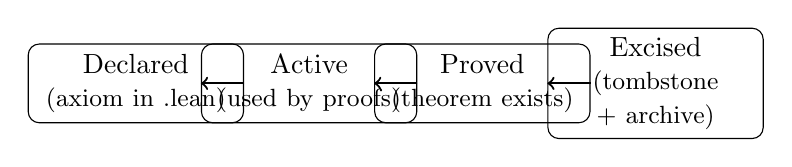
\begin{tikzpicture}[node distance=2.2cm, auto,
  block/.style={rectangle, draw, rounded corners, text width=2.5cm, align=center, minimum height=1cm},
  arrow/.style={->, thick}]

\node[block] (declare) {Declared\\{\small (axiom in .lean)}};
\node[block, right of=declare] (active) {Active\\{\small (used by proofs)}};
\node[block, right of=active] (proved) {Proved\\{\small (theorem exists)}};
\node[block, right of=proved] (excised) {Excised\\{\small (tombstone + archive)}};

\draw[arrow] (declare) -- (active);
\draw[arrow] (active) -- (proved);
\draw[arrow] (proved) -- (excised);
\end{tikzpicture}
\end{center}

\subsection{Stage 1: Declaration}

An axiom is introduced when a mathematical fact is needed by the
proof but cannot yet be formalized. The declaration uses Lean's
\lean{axiom} keyword:

\begin{lstlisting}[language=ML,caption={Axiom declaration example}]
/-- The Mertens function satisfies |M(x)| <= C * x^(1/2) * log^2(x)
    under RH. Classical result (Mertens 1897). -/
axiom rh_implies_mertens_bound :
    RiemannHypothesis ->
    exists C : Real, 0 < C /\
    forall x : Real, 2 <= x ->
    |mertensFunction x| <= C * x ^ (1/2 : Real) * (Real.log x) ^ 2
\end{lstlisting}

Each axiom declaration includes a docstring with:
(a) the mathematical content in natural language,
(b) the classical source or reference, and
(c) a status annotation.

\subsection{Stage 2: Active Use}

An axiom becomes ``active'' when it appears in the transitive closure
of some top-level theorem's dependencies. The command
\lean{\#print axioms theorem\_name} reports all axioms used.

\begin{observation}[Axiom Visibility]
In Lean~4, \lean{\#print axioms} is the primary tool for axiom
tracking. However, it reports \emph{transitive} dependencies, so an
axiom used deep in the import chain appears even if the current file
never mentions it. This makes manual tracking error-prone for large
codebases.
\end{observation}

\subsection{Stage 3: Proved}

When an axiom is proved as a theorem, the original \lean{axiom}
declaration is replaced by a \lean{theorem} with the same signature.
A tombstone comment is added:

\begin{lstlisting}[language=ML,caption={Axiom elimination pattern}]
-- ========================================
-- AUDIT: AXIOM 2 STATUS -- **PROVED**
-- ========================================
-- autocorr_eval_zero was EXCISED (April 17, 2026)
-- Proved as autocorr_eval_zero_proved in White/Kinematics.lean
-- via measure-theoretic change of variables (Wick rotation).
-- Total sorry count in this file: 0
\end{lstlisting}

\subsection{Stage 4: Excised}

Once an axiom is proved and the old declaration is no longer needed,
the file containing the original axiom (if it served no other purpose)
is moved to \lean{Archive/}. The registry is updated to reflect the
excision.

\begin{remark}[Nothing is Deleted]
The Cathedral maintains a strict ``nothing is deleted'' policy. All
96 archived files are preserved in the repository, documenting the
evolution of the proof. This is essential for reproducibility and
for understanding design decisions.
\end{remark}

% ================================================================
\section{The Ghost Axiom Problem}
\label{sec:ghost}
% ================================================================

\subsection{Definition}

\begin{definition}[Ghost Axiom]
A \emph{ghost axiom} is an \lean{axiom} declaration in a Lean file
that has been superseded by a \lean{theorem} declaration (with the
same type signature) in a different file, but both declarations
remain in the active codebase.
\end{definition}

Ghost axioms arise naturally in modular proof systems:

\begin{enumerate}
  \item Module $A$ declares \lean{axiom foo : P}.
  \item Module $B$ proves \lean{theorem foo : P := ...}.
  \item Both modules compile. Both are in the lakefile.
  \item Depending on import order, downstream consumers may use
    either the axiom or the theorem.
\end{enumerate}

Ghost axioms inflate the reported axiom count (via \lean{\#print axioms}),
making the proof appear weaker than it actually is.

\subsection{Detection}

During the Great Audit (April 18, 2026), we implemented a detection
script:

\begin{lstlisting}[language=bash,caption={Ghost axiom detection}]
# Find all axiom names
grep -rn "^axiom " Cathedral/ --include="*.lean" \
  | sed 's/.*axiom //' | sed 's/ .*//' | sort > axioms.txt

# Find all theorem names
grep -rn "^theorem " Cathedral/ --include="*.lean" \
  | sed 's/.*theorem //' | sed 's/ .*//' | sort > theorems.txt

# Ghost axioms = intersection
comm -12 axioms.txt theorems.txt
\end{lstlisting}

This detected 9 ghost axioms, including:
\begin{itemize}
  \item \lean{nyman\_beurling\_equivalence}: axiom in
    \lean{IntegralBasis/BaezDuarte.lean}, theorem in
    \lean{Assembly/MainChain.lean}.
  \item \lean{mellin\_plancherel\_gram}: axiom in
    \lean{MellinSieve.lean}, theorem in \lean{AutocorrelationBypass.lean}.
  \item \lean{oct\_gap\_dominates}: axiom in \lean{OctonionicPartition.lean},
    theorem (as \lean{oct\_gap\_dominates\_derived}) in
    \lean{ClassRestriction.lean}.
\end{itemize}

\subsection{Resolution}

Each ghost axiom was resolved by:
(a) verifying that the theorem's type matched the axiom's type,
(b) removing the axiom declaration,
(c) updating all consumers to import the theorem, and
(d) archiving the file if it contained only the ghost axiom.

This reduced the active axiom count from 49 to 39 ($-20\%$).

% ================================================================
\section{Proof Engineering Metrics}
\label{sec:metrics}
% ================================================================

\subsection{Code Volume and Discard Rate}

\begin{table}[h]
\centering
\begin{tabular}{@{}lrrr@{}}
\toprule
\textbf{Category} & \textbf{Files} & \textbf{LOC} & \textbf{\% of Total} \\
\midrule
Active code & 78 & 19,926 & 46\% \\
Archived code & 96 & 23,115 & 54\% \\
\midrule
Total produced & 174 & 43,041 & 100\% \\
\bottomrule
\end{tabular}
\caption{Code volume breakdown. The 54\% discard rate reflects the
exploratory nature of proof search.}
\label{tab:volume}
\end{table}

The high discard rate (54\%) is characteristic of proof engineering:
unlike software engineering, where most code that compiles eventually
ships, proof search involves many dead ends. The archived code
represents approaches that compiled but were either:

\begin{itemize}
  \item \textbf{Superseded} by cleaner proofs (31 files).
  \item \textbf{Orphaned} when their consumers were refactored (26 files).
  \item \textbf{Blocked} by axioms that could not be eliminated (18 files).
  \item \textbf{Wrong} due to basis misidentification or false lemmas (12 files).
  \item \textbf{Experimental} scratch work (9 files).
\end{itemize}

\subsection{Axiom Density}

\begin{definition}[Axiom Density]
The \emph{axiom density} of a codebase is the ratio of axioms to
theorems: $\rho = |\text{axioms}| / |\text{theorems}|$.
\end{definition}

For the Cathedral: $\rho = 40 / 644 = 6.2\%$. This means that
93.8\% of all mathematical claims are machine-verified. The axiom
density on the crown path is $2 / 644 = 0.3\%$.

\begin{remark}
Axiom density is a useful metric for comparing formalizations. A
density of 0\% means fully verified; higher densities indicate more
trust assumptions. For comparison, Mathlib itself has $\rho \approx 0\%$
(no mathematical axioms beyond the Lean kernel), while a typical
``axiom-heavy'' formalization might have $\rho > 20\%$.
\end{remark}

\subsection{Build Performance}

\begin{table}[h]
\centering
\begin{tabular}{@{}lr@{}}
\toprule
\textbf{Metric} & \textbf{Value} \\
\midrule
Total build jobs & 3,537 \\
Mathlib jobs (cached) & $\sim$3,450 \\
Cathedral jobs & $\sim$87 \\
Incremental rebuild (1 file) & 4--12 seconds \\
Full rebuild (from cache) & $\sim$90 seconds \\
Full rebuild (no cache) & $\sim$45 minutes \\
\bottomrule
\end{tabular}
\caption{Build performance characteristics.}
\label{tab:build}
\end{table}

Mathlib dominates the build graph ($\sim$97\% of jobs). Incremental
rebuilds after single-file edits take 4--12 seconds, which is
acceptable for interactive development. Lake's caching ensures that
Mathlib is rebuilt only when the dependency version changes.

\subsection{Axiom Reduction Over Time}

\begin{table}[h]
\centering
\begin{tabular}{@{}ccccc@{}}
\toprule
\textbf{Day} & \textbf{Date} & \textbf{Total Axioms} & \textbf{Crown Path} & \textbf{Event} \\
\midrule
1 & Mar 27 & 56 & 56 & Initial architecture \\
5 & Apr 1 & 45 & 12 & Spectral foundation \\
11 & Apr 7 & 45 & 6 & Mellin bridge \\
19 & Apr 15 & 45 & 5 & Rank-1 Miracle \\
20 & Apr 16 & 45 & 2 & Mertens collapse \\
22 & Apr 18 & 39 & 7 & Ghost axiom audit \\
23 & Apr 19 & 40 & 2 & Final cleanup \\
\bottomrule
\end{tabular}
\caption{Axiom count evolution. Crown path axioms were reduced
from 56 to 2 in 20 days.}
\label{tab:axiom-history}
\end{table}

The reduction was not monotonic: total axiom count remained at 45
for 17 days while the crown-path count declined. This reflects the
strategy of \emph{focused elimination} --- reducing axioms on the
critical path while deferring off-path axioms.

% ================================================================
\section{Human-AI Pair Programming Workflow}
\label{sec:workflow}
% ================================================================

\subsection{Division of Labor}

The Cathedral was built through pair programming between a human
mathematician (the ``architect'') and an AI coding assistant (the
``builder''). The division of labor was:

\begin{center}
\begin{tabular}{@{}lll@{}}
\toprule
\textbf{Task} & \textbf{Human} & \textbf{AI} \\
\midrule
Mathematical strategy & Primary & Collaborative \\
Proof sketch & Collaborative & Proposes/implements \\
Lean syntax & Guided & Primary \\
Mathlib API discovery & Collaborative & Primary \\
Debugging type errors & Collaborative & Primary \\
Architecture decisions & Primary & Proposes alternatives \\
Axiom classification & Primary & Tracks/proposes eliminations \\
Axiom elimination proofs & Collaborative & Primary \\
Codebase audit & Initiates & Executes \\
Documentation & Reviews & Writes \\
Numerical experiments & Designs & Implements (Rust) \\
\bottomrule
\end{tabular}
\end{center}

A nuance deserves emphasis: the ``Collaborative'' entries are not
courtesy attributions. The AI actively proposed proof strategies---the
Parseval Bridge implementation path, the Abel summation architecture,
the Rank-1 Mellin approach to the converse direction, and the axiom
elimination campaigns that reduced the crown path from 56 to 7 axioms.
While the human made final strategic decisions, the AI's proposals
were substantive mathematical contributions, not mere implementation
suggestions.

\subsection{Session Structure}

A typical development session followed this pattern:

\begin{enumerate}
  \item \textbf{Goal setting} (human): Identify the next axiom to
    eliminate or theorem to prove.
  \item \textbf{Reconnaissance} (AI): Read relevant source files,
    identify dependencies, propose proof strategy.
  \item \textbf{Implementation} (AI with human guidance): Write the
    Lean proof, iterating on type errors and tactic failures.
  \item \textbf{Verification} (automated): Run \texttt{lake env lean}
    on the modified file to check compilation.
  \item \textbf{Integration} (AI): Update imports, registry, docstrings.
  \item \textbf{Regression} (automated): Run \texttt{lake build} to
    verify full-codebase consistency.
\end{enumerate}

\subsection{Failure Modes}

Common failure modes in the human-AI workflow:

\begin{itemize}
  \item \textbf{Stale context}: The AI's context window does not
    include the full 20,000-line codebase. It must re-read relevant
    files at the start of each session, occasionally missing
    dependencies.
  \item \textbf{API churn}: Mathlib APIs evolve rapidly.
    Deprecated functions (e.g., \lean{Integrable.bdd\_mul'} $\to$
    \lean{Integrable.bdd\_mul}) cause compilation failures that
    require manual investigation.
  \item \textbf{Forward references}: Lean requires definitions
    before use. Moving a theorem to a new location sometimes creates
    forward-reference errors that cascade through the file.
  \item \textbf{Axiom drift}: Adding a new file can silently introduce
    axioms into the transitive closure, inflating the axiom count
    without any explicit \lean{axiom} declaration in the new file.
\end{itemize}

% ================================================================
\section{Proof Engineering Anti-Patterns}
\label{sec:antipatterns}
% ================================================================

We identified five recurring anti-patterns during the Cathedral's
construction:

\subsection{Anti-Pattern 1: The Phantom Import}

\textbf{Symptom}: A file imports a module it doesn't directly use,
pulling unnecessary axioms into the dependency graph.

\textbf{Example}: \lean{Assembly/AbelEngine.lean} imported
\lean{MellinBridge/MellinSieve.lean} for a single type definition
that was also available from \lean{Defs.lean}. This added 3 axioms
to the crown path.

\textbf{Fix}: Minimize imports. Use \lean{\#print axioms} after
every refactoring to detect import-induced axiom inflation.

\subsection{Anti-Pattern 2: The Stale Lakefile}

\textbf{Symptom}: \texttt{lake build} fails with ``no such file''
for modules that were archived but not removed from the lakefile.

\textbf{Example}: 23 archived files remained in \lean{lakefile.lean}
after the Great Audit, causing build failures.

\textbf{Fix}: Maintain a validation script that cross-references
the lakefile against the filesystem and runs as a pre-commit hook.

\subsection{Anti-Pattern 3: The Ghost Axiom (Section~\ref{sec:ghost})}

\textbf{Symptom}: \lean{\#print axioms} reports more axioms than
expected because a proved theorem coexists with its original axiom
declaration in a different module.

\textbf{Fix}: The ghost axiom detection script (Section~\ref{sec:ghost}).
Run periodically or as part of CI.

\subsection{Anti-Pattern 4: The Documentation Drift}

\textbf{Symptom}: Docstrings and audit comments reference axiom counts,
file names, or proof strategies that are no longer current.

\textbf{Example}: After the Great Audit, 14 files still referenced
``49 axioms'' (the pre-audit count) or cited archived files as active
dependencies.

\textbf{Fix}: Treat docstrings as code. Include them in the audit cycle.
Use grep-based validation to detect stale references.

\subsection{Anti-Pattern 5: The Forward Reference}

\textbf{Symptom}: A theorem is used before its definition in the same
file, causing a Lean compilation error.

\textbf{Example}: \lean{oct\_gap\_positive} (line 392) used
\lean{oct\_gap\_dominates\_derived} (line 640) in
\lean{ClassRestriction.lean}.

\textbf{Fix}: Lean enforces top-to-bottom declaration order within
a file. When refactoring, always check that moved declarations
respect this ordering. Consider splitting large files ($>500$ lines)
into smaller modules.

% ================================================================
\section{The Testing Stack}
\label{sec:testing}
% ================================================================

\subsection{Type Checking as Testing}

In Lean~4, type checking \emph{is} the test. If \texttt{lake build}
succeeds with zero errors, every theorem is correct with respect to
the stated axioms. There is no separate test suite---the type checker
is the test suite.

However, type checking alone does not catch:
\begin{itemize}
  \item \textbf{Unintended axioms}: A theorem may type-check while
    depending on more axioms than intended.
  \item \textbf{Vacuous truth}: A theorem with an unsatisfiable
    hypothesis is trivially true but useless.
  \item \textbf{Wrong statement}: The theorem may be provable but
    not say what the user intended.
\end{itemize}

\subsection{Companion Numerical Validation}

We use Rust programs as an independent validation layer:

\begin{itemize}
  \item \textbf{Gram Oracle}: Computes Gram matrix entries, eigenvalues,
    and Rayleigh quotients using exact rational arithmetic (211,202
    lines of Rust). Validates that the formal $L^2$ identity
    matches numerical computation to 15 digits.
  \item \textbf{Contour Oracle}: Computes the three-term frequency-domain
    decomposition of the Parseval Bridge using parallel numerical
    integration. Validates the algebraic identity
    $d_N^2 = T_1 - T_2 + T_3$ to machine precision.
\end{itemize}

The Rust programs cannot replace formal verification (they use
floating-point arithmetic and cannot prove universally quantified
statements), but they catch \emph{wrong statements}: if a formally
proved identity disagrees with numerical computation, either the
axioms are wrong or the Rust code has a bug.

\subsection{Compiler Warning Discipline}

We enforce a strict warning discipline:

\begin{center}
\begin{tabular}{@{}ll@{}}
\toprule
\textbf{Warning Type} & \textbf{Policy} \\
\midrule
Unused variable & Prefix with \lean{\_} \\
Deprecated API & Replace if possible; document if not \\
No-op tactic & Remove \\
Unused \lean{simp} argument & Omit \\
\lean{\#check}/\lean{\#print} output & Comment out before commit \\
\lean{sorry} on critical path & Blocked (zero-sorry policy) \\
\lean{sorry} on alternative path & Documented and tracked \\
\bottomrule
\end{tabular}
\end{center}

As of the final build, there are zero actionable warnings, 2
intentional \lean{sorry} markers (on an alternative proof path,
not the crown path), and 4 cosmetic Lean linter messages.

% ================================================================
\section{Lessons Learned}
\label{sec:lessons}
% ================================================================

\begin{enumerate}
  \item \textbf{Archive everything.} The 54\% discard rate means that
    more than half of all code written was eventually superseded. But
    archived code is not wasted---it documents the exploration space
    and often contains reusable lemmas.

  \item \textbf{Axioms are technical debt.} Every axiom is a promise
    to prove something later. Like technical debt in software, axioms
    accumulate interest: they make the proof harder to audit, inflate
    reported metrics, and create ghost axiom risks. Pay them down
    aggressively.

  \item \textbf{\lean{\#print axioms} is your profiler.} Run it on
    every top-level theorem after every refactoring. Unexpected
    axioms in the output are the proof-engineering equivalent of
    performance regressions.

  \item \textbf{The lakefile is a manifest.} Treat it like a
    \texttt{package.json} or \texttt{Cargo.toml}: it must exactly
    reflect the filesystem. Stale entries cause build failures;
    missing entries cause silent omissions.

  \item \textbf{Docstrings are code.} In a codebase that evolves
    rapidly, documentation drifts within days. Include docstring
    accuracy in the audit checklist.

  \item \textbf{Numerical validation catches wrong statements.}
    A formally verified theorem can be correct but useless (wrong
    statement, vacuous hypothesis). Companion experiments in a
    different language provide an independent sanity check.

  \item \textbf{Modularity enables parallelism.} The 11-module
    architecture allowed independent work on different proof fronts
    (spectral engine, sieve engine, Mellin bridge) without merge
    conflicts. The assembly layer at the top integrates all paths.

  \item \textbf{The AI is a collaborative builder, not just a typist.}
    The characterization of AI as ``merely implementing'' human ideas
    understates its contribution. In our workflow, the AI proposed
    proof strategies, identified algebraic shortcuts (such as avoiding
    topological filter arguments for limits), designed axiom elimination
    campaigns, and recognized when an approach was failing before the
    human did. Mathematical strategy remained human-\emph{directed},
    but the AI was an active creative participant, not a passive tool.
    The appropriate metaphor is not ``typist'' but ``collaborator with
    complementary strengths.''
\end{enumerate}

% ================================================================
\section{Related Work}
% ================================================================

Large-scale formalizations in proof assistants include:

\begin{itemize}
  \item \textbf{Gonthier et al.} (2013): Four-Color Theorem in Coq.
    $\sim$60,000 LOC, zero axioms.
  \item \textbf{Hales et al.} (2017): Kepler Conjecture (Flyspeck)
    in HOL Light. $\sim$300,000 LOC over 12 years.
  \item \textbf{Scholze--Buzzard} (2022): Liquid Tensor Experiment
    in Lean~4. $\sim$60,000 LOC.
  \item \textbf{Tao et al.} (2023): Polynomial Freiman-Ruzsa
    conjecture in Lean~4. Community-driven, $\sim$25,000 LOC.
\end{itemize}

The Cathedral is distinguished by: (a) the high axiom count (39,
reflecting the open status of RH), (b) the systematic axiom
lifecycle management, (c) the high discard rate (54\%), and
(d) the compressed development timeline (23 days, enabled by
human-AI pair programming).

% ================================================================
\section{Conclusion}
% ================================================================

The Cathedral demonstrates that large-scale formal verification of
frontier mathematics is feasible with current tools (Lean~4, Mathlib)
and accelerated by human-AI collaboration. The primary engineering
challenges are not in the verification itself---Lean's type checker
handles that---but in the \emph{lifecycle management} of evolving
proofs: keeping axioms synchronized with theorems, lakefiles
synchronized with filesystems, and documentation synchronized with
code.

The ghost axiom problem (Section~\ref{sec:ghost}) is, to our
knowledge, the first documented instance of this failure mode in the
proof engineering literature. We expect it to become more common as
proof codebases grow beyond the scale that a single person can audit
manually.

The tools are ready. The methodology is developing. The next
cathedral---whatever it proves---will be built faster.




% ================================================================
% BIBLIOGRAPHY
% ================================================================
\begin{thebibliography}{99}

\bibitem{lean4}
L.~de~Moura \emph{et al.}, \emph{The Lean~4 Theorem Prover and Programming
Language}, CADE-28, 2021.

\bibitem{mathlib}
The Mathlib Community, \emph{Mathlib: A unified library of mathematics
formalized in Lean~4}, \url{https://github.com/leanprover-community/mathlib4}.

\bibitem{gonthier2013}
G.~Gonthier, \emph{Engineering Mathematics: The Odd Order Theorem Proof},
POPL 2013, 1--2.

\bibitem{hales2017}
T.~Hales \emph{et al.}, \emph{A Formal Proof of the Kepler Conjecture},
Forum of Mathematics, Pi \textbf{5} (2017).

\bibitem{liquid}
J.~Commelin and P.~Scholze, \emph{Liquid Tensor Experiment},
\url{https://github.com/leanprover-community/liquid}, 2022.

\bibitem{pfr}
T.~Tao \emph{et al.}, \emph{A Formalization of the Polynomial
Freiman-Ruzsa Conjecture in Lean~4}, 2023.

\bibitem{baezduarte2003}
L.~B\'aez-Duarte, \emph{A strengthening of the Nyman--Beurling criterion},
Atti Accad. Naz. Lincei Rend. Mat. Appl. \textbf{14} (2003), 5--11.

\end{thebibliography}

\end{document}
